\chapter{Proposed System and Implementation}\label{ch:proposed}

\section{Requirements}
\begin{table}[H]
\centering
\caption{Functional (FR) and non-functional (NFR) requirements.}\label{tab:req}
\begin{small}
\begin{tabularx}{\textwidth}{@{}lY@{}}
\toprule
\textbf{ID} & \textbf{Requirement}\\
\midrule
FR1 & Accept a JPG or PNG field photo and the crop name; reject empty or corrupt files with a clear message.\\
FR2 & Detect and segment plants zero-shot with Grounding DINO and SAM~2 on the local GPU.\\
FR3 & Spray only zones approved by the deterministic gate; list every withheld plant with its reason.\\
FR4 & Suppress the whole map when the photo is mostly weed (above 85\% infestation): spot spraying is the wrong tool there.\\
FR5 & Optionally review withheld plants with the escalation agent; its verdict is advice, the gate still decides.\\
FR6 & Give herbicide advice only from the ICAR bulletin row for the declared crop and weed; otherwise say ``no evidence''.\\
FR7 & Export approved zones as GeoJSON~\cite{rfc7946}, one feature per zone, clearly marked as not GPS.\\
FR8 & Summarise the result for a farmer in English, Hindi or Marathi without adding any advice.\\
NFR1 & Honesty: every screen says REAL or MOCK; a real run that cannot load a model fails loudly instead of showing fake output.\\
NFR2 & Safety: any error, missing evidence or disagreement means ``do not spray''.\\
NFR3 & Speed: under 1~s per photo on the laptop GPU after the models are loaded.\\
NFR4 & Hardware: fit in 8~GB of GPU memory; reasoning models run in the cloud on free tiers.\\
NFR5 & Testability: deterministic results; all rules unit tested; CI on every push.\\
\bottomrule
\end{tabularx}
\end{small}
\end{table}

\section{Architecture}
AgriAgent follows a ``two systems'' design. \emph{System~1} is fast and local: detection, segmentation,
the plant rules and the deterministic gate, all on the laptop. \emph{System~2} is slow and deliberate:
cloud vision-language models that explain, advise and review, but never decide alone.
Figure~\ref{fig:arch} shows the pipeline.

\begin{figure}[H]
\centering
\begin{tikzpicture}[
  node distance=5mm,
  box/.style={draw=accent,rounded corners=2pt,fill=accent!8,text width=12.2cm,inner sep=5pt,font=\small,align=left},
  gate/.style={box,fill=yellow!15,draw=orange!70!black},
  cloud/.style={box,fill=blue!6,draw=blue!50!black,text width=5.85cm},
  io/.style={box,fill=black!4,draw=black!50},
  arr/.style={-{Stealth[length=2.5mm]},thick,accent}]
\node[io] (in) {\textbf{Input:} RGB field photo + declared crop (sugar beet, cotton, wheat, rice). Prompt \code{weed . <crop> plant .}};
\node[box,below=of in] (det) {\textbf{1 Detect} -- Grounding DINO-tiny (local GPU): boxes, each with a label taken from the prompt words and a confidence score.};
\node[box,below=of det] (seg) {\textbf{2 Segment} -- SAM~2-tiny (local GPU): one mask per box with a predicted quality score; re-prompted with a corrective point when quality $<0.85$.};
\node[box,below=of seg] (rules) {\textbf{3 Plant rules (frozen v3)} -- every green patch is classified crop / weed / unsure by four plain rules: crop-mask overlap, planting row, size relative to the crop, off-row.};
\node[gate,below=of rules] (gate) {\textbf{4 Safety gate (deterministic, final authority)} -- spray a zone only if it is a weed by label policy (confidence $\ge 0.70$, quality $\ge 0.85$) or by the plant rules; never a crop word or a mixed label; suppress the map above 85\% infestation. Everything else is withheld with a reason.};
\node[cloud,below=of gate.south west,anchor=north west] (agent) {\textbf{5a Escalation agent} (optional) -- per withheld plant: row rule $\rightarrow$ Clef Flash $\rightarrow$ Qwen~3.8 VLM under a call budget; advice only.};
\node[cloud,below=of gate.south east,anchor=north east] (sys2) {\textbf{5b System~2 + ICAR} -- Qwen~3.8 names the weed; the herbicide comes only from the ICAR bulletin row for the declared crop.};
\node[io,below=of agent.south west,anchor=north west,yshift=-1mm] (out) {\textbf{Output:} Streamlit app (REAL/MOCK banner, approved zones only), GeoJSON spray map, farmer summary (EN/HI/MR).};
\draw[arr] (in) -- (det); \draw[arr] (det) -- (seg); \draw[arr] (seg) -- (rules); \draw[arr] (rules) -- (gate);
\draw[arr] (gate.south -| agent.north) -- (agent.north); \draw[arr] (gate.south -| sys2.north) -- (sys2.north);
\draw[arr] (agent.south) -- (agent.south |- out.north); \draw[arr] (sys2.south) -- (sys2.south |- out.north);
\end{tikzpicture}
\caption{AgriAgent pipeline. Green: local, deterministic or pretrained; yellow: the safety gate; blue: cloud models that advise only.}\label{fig:arch}
\end{figure}

\section{The safety gate}\label{sec:gate}
The gate is the only component allowed to approve a spray zone (modules
\code{deterministic\_\allowbreak router.py} and \code{workflow.py}). Its rules are deliberately plain so that each can be unit tested and
explained; Section~\ref{sec:math-gate} states them as equations.
\begin{itemize}
\item \textbf{Label policy.} A detector mask is a spray candidate only if its label names a weed.
  Labels that name the crop, or mix crop and weed words (Grounding DINO sometimes returns ``weed sugar
  beet plant''), are withheld.
\item \textbf{Confidence and quality.} The detector score must be at least 0.70 and SAM~2's predicted
  mask quality at least 0.85. The application's slider may raise the confidence floor, never lower it.
\item \textbf{Not one plant.} A mask covering more than half of the photo is withheld: it is the whole
  field, not a weed.
\item \textbf{Infestation ceiling.} If approved zones cover more than 85\% of the photo, the whole map
  is suppressed.
\item \textbf{Plant-rule zones.} Patches the plant rules call ``weed'' are approved after every crop
  pixel has been removed from them; ``unsure'' patches never are.
\item \textbf{Fail safe.} Any exception, missing input or missing evidence results in withholding,
  never spraying.
\end{itemize}
An early version passed confidence and quality to the gate hard-coded as 1.0, so every ``weed'' was
sprayed; the bug was found in our code review and fixed before any measurement.

\section{Plant rules (v3, frozen)}\label{sec:rules}
Grounding DINO rarely boxes the small weeds: in our sugar beet photos it boxes mostly the large crop
plants (Section~\ref{sec:cheap}). Its boxes therefore cannot be the only spray candidates. The plant
rules (\code{src/vision/plant\_candidates.py}) take every connected patch of vegetation, found by
thresholding the excess-green index~\cite{woebbecke1995color} with a per-photo Otsu
threshold~\cite{hamuda2016survey} after closing small gaps between the leaves of one plant, and
classify it, in this order:
\begin{enumerate}
\item \textbf{crop} if at least 30\% of the patch lies inside a SAM~2 mask that the detector labelled as the crop;
\item \textbf{crop} if the photo shows clear planting rows and the patch lies on a dense row band;
\item \textbf{weed} if the photo has crop masks and the patch is smaller than a quarter of the median
  crop plant in the same photo (self-calibrating; no threshold was tuned on labels), otherwise
  \textbf{unsure};
\item \textbf{weed} if the photo has no crop masks but clear rows, and the patch lies off the row band;
\item \textbf{unsure} otherwise, which is never sprayed.
\end{enumerate}
Rules 2 and 4 use the row structure in the same spirit as the row-based labelling of Bah et
al.~\cite{bah2018unsupervised} and Louargant et al.~\cite{louargant2018rowcrops}. The rules were developed
on the 30 development photos and then frozen as ``v3'' before a single run on the 90 held-out photos.
Rule~4 is also the main known weakness (finding F1, Section~\ref{sec:f1}).

\section{The escalation agent}\label{sec:agent}
The only agent in AgriAgent (\code{src/agents/escalation\_agent.py}) reviews plants the gate withheld,
largest first, up to three per photo. For each plant it gathers evidence from the cheapest source to
the most expensive: the row rule, then Cloudflare's Clef Flash decision model~\cite{doc_cloudflare},
then the Qwen~3.8 27B vision-language model shown a crop of the plant. It stops when the evidence is
decisive or its call budget is spent. A source's stated confidence is not its accuracy, so each answer
is weighted by the source's accuracy measured on 20 labelled patches, and the answers are combined as
in a naive Bayes classifier (Section~\ref{sec:math-agent}). One source alone can never reach a
verdict; two that agree can; sources that disagree cancel out to ``unsure''. The agent returns a trace
of every call, so each verdict can be explained, and its verdict is advice: the gate still decides.

\section{System~2 and ICAR herbicide advice}
When the detections are uncertain, or when the user asks, System~2 shows the photo to Qwen~3.8 27B and
asks for the crop, the weed and the growth stage. The herbicide then comes only from a table
transcribed from the ICAR--DWR bulletin \emph{Herbicide Use in Indian Agriculture}~\cite{choudhury2016icar}
(\code{src/agronomy/knowledge\_store.py}), and only from the row for the declared crop and a matching
weed. Doses are clamped to the bulletin's maximum, and banned, withdrawn and refused herbicides (bulletin
Table~3.3) are rejected. If no row matches, the screen says ``no evidence'' instead of guessing. Every
row was checked against the PDF (Section~\ref{sec:icar}).

\section{Farmer summary}
A short plain-language summary is built only from the pipeline's own facts (zones sprayed, plants left
unsure, the prescription). A language model may reword it in Hindi or Marathi, with a fixed glossary
for crop and weed names. It is rejected, and the English template shown, if it fails or mentions a
dose when no prescription exists. Safety sentences (the wrong-crop warning and ``this is a suggestion,
read the label'') are fixed translated text appended after the model's wording, never left to the
model.

\section{Datasets}\label{sec:datasets}
\begin{table}[H]
\centering
\caption{Data sources and links.}\label{tab:datasets}
\begin{small}
\begin{tabularx}{\textwidth}{@{}L{3.1cm}YL{2.6cm}@{}}
\toprule
\textbf{Dataset} & \textbf{Contents and link} & \textbf{Used for}\\
\midrule
sugarbeets\-And\-weeds \cite{data_sugarbeets} & 120 photos, 512$\times$512, Pascal VOC boxes for sugar beet and weed. The images resemble the Bonn sugar beet data~\cite{chebrolu2017sugarbeet}; the uploader does not document the origin. \url{https://www.kaggle.com/datasets/wangyongkun/sugarbeetsandweeds} & 30 development + 90 held-out photos\\
Cotton\-Weed\-Det3 \cite{data_cottonweeddet3,rahman2023cotton} & Cotton field photos with boxes for three weeds (palmer amaranth, morningglory, waterhemp); cotton itself is never labelled. \url{https://www.kaggle.com/datasets/yuzhenlu/cottonweeddet3} & 8 development photos\\
ICAR--DWR bulletin No.~22~\cite{choudhury2016icar} & Approved herbicides per crop with dose, water volume and waiting period; list of banned herbicides. \url{https://dwr.icar.gov.in} & System~2 knowledge store\\
\bottomrule
\end{tabularx}
\end{small}
\end{table}

\section{Technology stack and hardware}
\begin{table}[H]
\centering
\caption{Technology stack.}\label{tab:stack}
\begin{small}
\begin{tabularx}{\textwidth}{@{}lY@{}}
\toprule
\textbf{Layer} & \textbf{Choice}\\
\midrule
Language & Python 3.11--3.13; type hints checked with mypy; style with ruff.\\
Vision models & \code{IDEA-Research/grounding-dino-tiny} and \code{facebook/sam2-hiera-tiny} through Hugging Face Transformers~\cite{doc_transformers}; PyTorch 2.11 with CUDA 12.8.\\
Reasoning models & Qwen~3.8 27B (\code{@cf/qwen/qwen3.8-27b}) and Clef Flash on Cloudflare Workers AI (free tier)~\cite{doc_cloudflare}; Groq~\cite{doc_groq} as an alternative provider.\\
Application & Streamlit~\cite{doc_streamlit}; GeoJSON export~\cite{rfc7946}.\\
Testing and CI & Python \code{unittest}; Streamlit \code{AppTest} for headless application tests; GitHub Actions on Python 3.11 and 3.13.\\
Hardware & Laptop with an NVIDIA RTX~5050 (8~GB) and 15~GB RAM. Both vision models together peak at about 2.4~GB of GPU memory; the system was also tested on an RTX~3050 (4~GB).\\
\bottomrule
\end{tabularx}
\end{small}
\end{table}

\section{Code structure}
\begin{table}[H]
\centering
\caption{Main modules.}\label{tab:modules}
\begin{small}
\begin{tabularx}{\textwidth}{@{}>{\raggedright\arraybackslash\footnotesize}p{6.2cm}Y@{}}
\toprule
\textbf{Module} & \textbf{Responsibility}\\
\midrule
\code{src/vision/grounding\_dino.py} & Detector wrapper: prompt to boxes; mock mode for tests; fails loudly if real weights cannot load.\\
\code{src/vision/sam2\_wrapper.py} & Boxes to masks with predicted quality; corrective-point refinement.\\
\code{src/vision/model\_cache.py} & Loads each real model once per process under a lock.\\
\code{src/vision/plant\_candidates.py} & Plant rules v3 (Section~\ref{sec:rules}).\\
\code{src/workflow.py} & \code{VisionWorkflowRunner}: detect, segment, refine, spray map with the gate, triage, System~2.\\
\code{src/agents/\allowbreak deterministic\_\allowbreak router.py} & Safety gate rules.\\
\code{src/agents/escalation\_agent.py} & Escalation agent and its three evidence sources.\\
\code{src/agronomy/} & System~2 reasoner, ICAR knowledge store, prescription and dose ceilings, providers, farmer summary.\\
\code{src/evaluation/} & Metrics: crop pixels sprayed, weed recall, savings, IoU/Dice; benchmark runner.\\
\code{app/} & Streamlit dashboard, KPI cards, visualisation, GeoJSON export.\\
\code{scripts/} & Baseline runner, manifest builders, provider check, verification and release scripts.\\
\code{tests/} & 235 unit tests and 35 end-to-end tests.\\
\bottomrule
\end{tabularx}
\end{small}
\end{table}

\section{Real and mock modes}
Every model wrapper has a mock mode that returns deterministic synthetic output, so that the
application and the tests run on any laptop without the 1.5~GB of weights. Early in the project, a
failed model load silently switched to mock output, and the application presented a mock diagnosis as
``verified''. Both were fixed: a real run that cannot load a model now raises an error, and every
result screen carries a REAL or MOCK banner. Mock mode never calls a cloud model.

\section{Application}
The Streamlit dashboard (\code{app/app.py}) takes a photo upload, the crop, the prompt, the confidence
slider (0.70 or higher), the nozzle buffer in pixels and two switches: force System~2, and review
unsure plants with the escalation agent (real mode, off by default). It shows the REAL/MOCK banner, a
wrong-crop warning when no plant matched the declared crop, KPI cards (area sprayed, herbicide saved,
zones), the photo beside the spray map with approved zones filled and outlined, the System~2 report,
the farmer summary and a GeoJSON download. An optional view colours every plant by the decision
taken: red sprayed, green protected as crop, yellow left alone (Figure~\ref{fig:verdict}). The last
result is cached against the photo and the settings, so changing the summary language or downloading
does not rerun the models.

\begin{figure}[H]
\centering
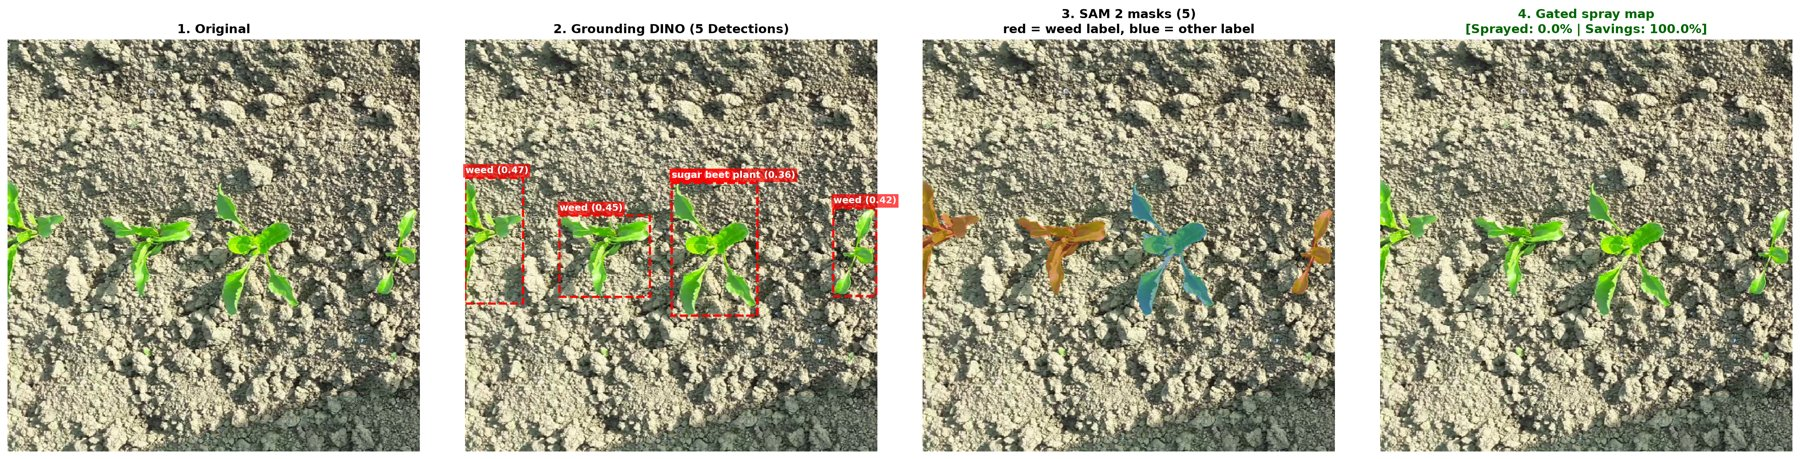
\includegraphics[width=0.95\textwidth]{real_run_beet_after_gate_fix}
\caption{Real run on a sugar beet photo (17 October, after the gate fix): photo, detector boxes, masks
and the spray map. All detector confidences were 0.36--0.47, below the 0.70 gate, so nothing was
sprayed: the crop is safe, but the weeds are missed. This is the Grounded SAM baseline behaviour that
the plant rules address.}\label{fig:gate}
\end{figure}

\begin{figure}[H]
\centering
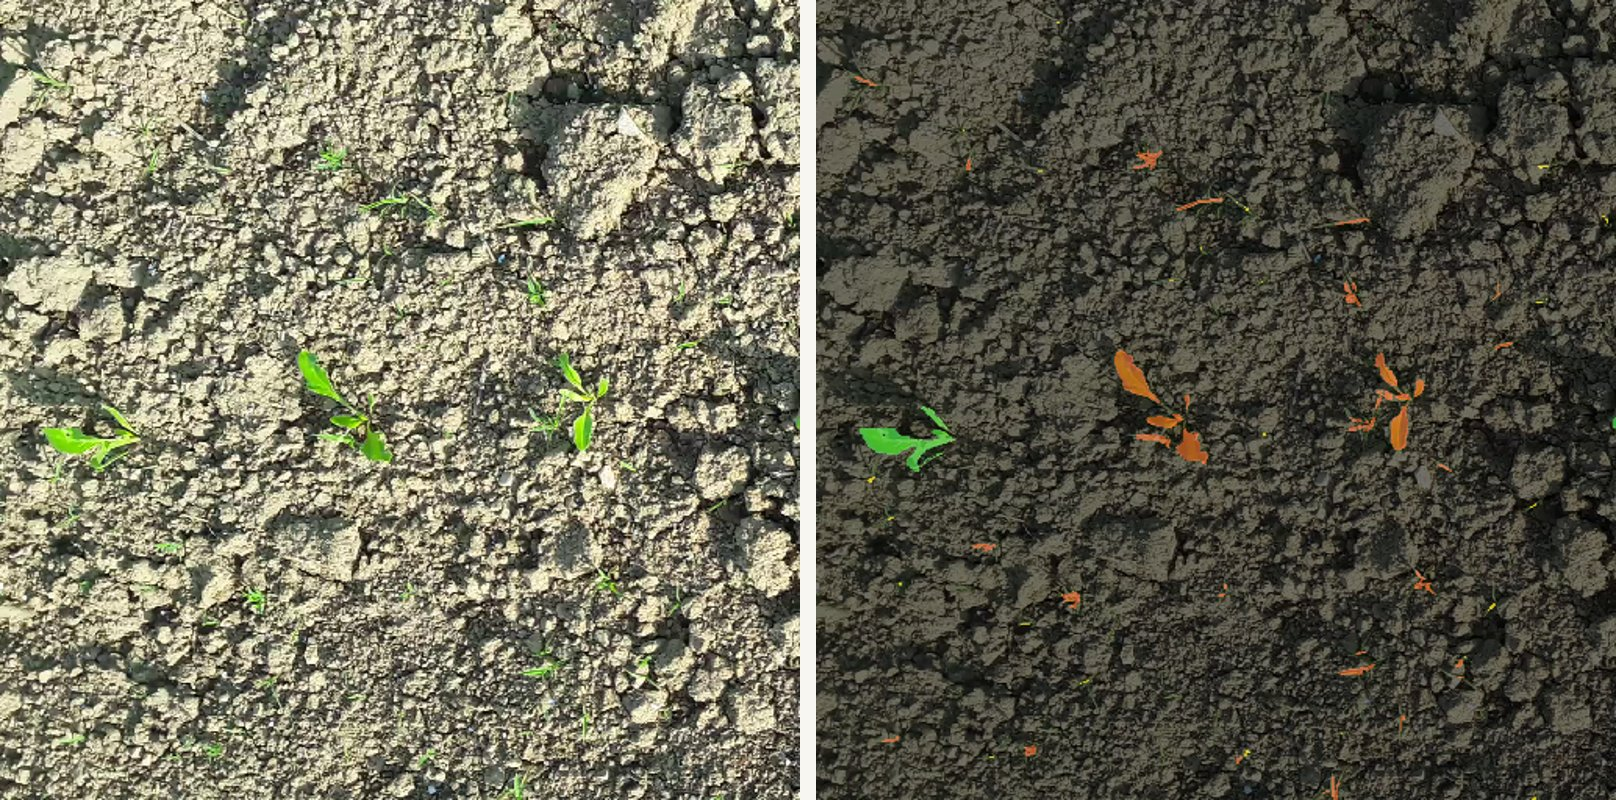
\includegraphics[width=0.49\textwidth]{verdict_beet_X2-30-0}\hfill
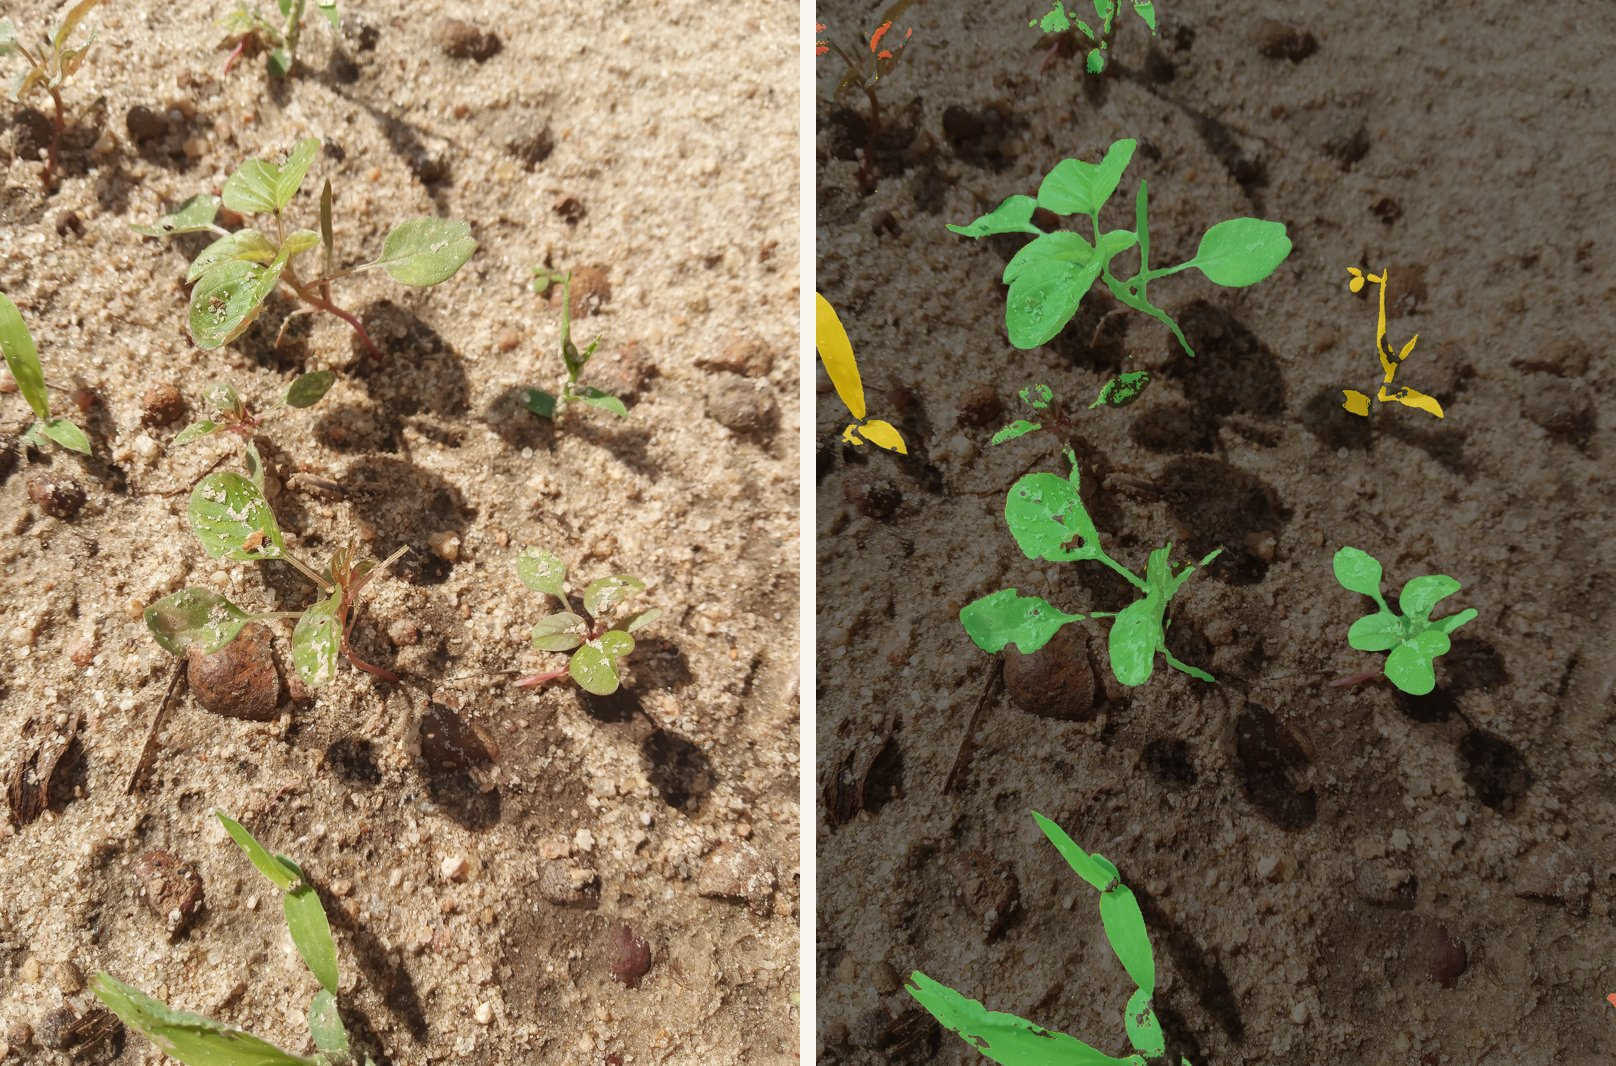
\includegraphics[width=0.49\textwidth]{verdict_cotton_CM_17}
\caption{The application's verdict view: red sprayed, green protected as crop, yellow left alone.
Left: sugar beet X2-30-0, where two of the three beets (centre and right) are wrongly sprayed; whole-beet
errors of this kind are analysed in Section~\ref{sec:f1}. Right: cotton CM\_17, where the detector boxed the large weeds as cotton,
so they were protected.}\label{fig:verdict}
\end{figure}

\section{GeoJSON export}
Each approved zone becomes one MultiPolygon feature traced along the exact pixel boundary of its mask,
with holes kept. Fragments under 16 pixels are dropped (jagged mask edges once produced 1,394 features
for three weeds). The top-left corner of the photo is pinned to a placeholder point at VJTI and each
pixel is taken as 5~mm on the ground; image rows grow downward and latitude northward, so rows are
subtracted. The file's metadata states that the coordinates are not GPS. Herbicide fields appear only
when System~2 produced a real prescription.
